%!TEX TS-program = xelatex
\documentclass[14pt, a4paper]{article}


%%%%%%%%%% Математика %%%%%%%%%%
\usepackage{amsmath,amsfonts,amssymb,amsthm,mathtools}



%%%%%%%%%%%%%%%%%%%%%%%% Шрифты %%%%%%%%%%%%%%%%%%%%%%%%%%%%%%%%%
\usepackage{fontspec}         % пакет для подгрузки шрифтов
\setmainfont{Arial}   % задаёт основной шрифт документа

% Команда, которая нужна для корректного отображения длинных тире и некоторых других символов.
\defaultfontfeatures{Mapping=tex-text}

% why do we need \newfontfamily:
% http://tex.stackexchange.com/questions/91507/
\newfontfamily{\cyrillicfonttt}{Arial}
\newfontfamily{\cyrillicfont}{Arial}
\newfontfamily{\cyrillicfontsf}{Arial}

\usepackage{unicode-math}     % пакет для установки математического шрифта
\setmathfont{Asana Math}      % шрифт для математики


\usepackage{polyglossia}      % Пакет, который позволяет подгружать русские буквы
\setdefaultlanguage{russian}  % Основной язык документа
\setotherlanguage{english}    % Второстепенный язык документа


%%%%%%%%%% Работа с картинками %%%%%%%%%
\usepackage{graphicx}                  % Для вставки рисунков
\usepackage{graphics}

\usepackage{float}               % возможность позиционировать объекты в нужном месте

%%%%%%%%%% Гиперссылки %%%%%%%%%%
\usepackage{xcolor}              % разные цвета
\usepackage{hyperref}
\hypersetup{
    unicode=true,           % позволяет использовать юникодные символы
    colorlinks=true,       	% true - цветные ссылки, false - ссылки в рамках
    urlcolor=blue,          % цвет ссылки на url
    linkcolor=red,          % внутренние ссылки
    citecolor=green,        % на библиографию
	pdfnewwindow=true,      % при щелчке в pdf на ссылку откроется новый pdf
	breaklinks              % если ссылка не умещается в одну строку, разбивать ли ее на две части?
}

\usepackage{setspace}
\usepackage[paper=a4paper,top=10mm, bottom=10mm,left=35mm,right=35mm,includefoot,includehead]{geometry}
\setstretch{1}  % Межстрочный интервал
\usepackage{extsizes} %чтобы подгрузить 14 шрифт
\setlength{\parskip}{4mm}   % Расстояние между абзацами
\usepackage{titlesec}


\usepackage{fancyhdr} % Колонтитулы
\pagestyle{fancy}

\titleformat{\section}
      {\Large\bfseries}
      {Приложение \Asbuk{section}:}{0.1 em}{}

\renewcommand{\headrulewidth}{0.2pt}  % Толщина линий, отчеркивающих верхний колонтитул
\renewcommand{\sectionmark}[1]{\markboth{%
\MakeUppercase{Приложение \Asbuk{section} \hspace{1em}#1}}{}}
	\rhead{ \thepage }
 	\lhead{\leftmark}
	\cfoot{Школа Чародейства и Волшебства <<Хогвартс>>} % номер страницы
	
\usepackage{afterpage}

\begin{document}

\afterpage{
\thispagestyle{empty}

\begin{figure}[t]
\begin{center}

\includegraphics[height=6cm,width=8cm,keepaspectratio]{herb.jpg}
\end{center}
\end{figure}

\vspace{1cm}

{\fontsize{12}{1}\selectfont \noindent Дорогой мистер Поттер!}

\vspace{2.5cm}

\noindent Мы рады проинформировать Вас, что Вам предоставлено место в Школе чародейства и волшебства «Хогвартс». Пожалуйста, ознакомьтесь с приложенным к данному письму списком необходимых книг и предметов. \\
\noindent Занятия начинаются 1 сентября. Ждем вашу сову не позднее 31 июля. \\
\noindent Искренне Ваша, \\
\noindent Минерва МакГонагалл \\
\noindent {\fontspec{Scrawl}{Minerva McGonagall}} \\
\noindent заместитель директора!


\center{ШКОЛА ЧАРОДЕЙСТВА И ВОЛШЕБСТВА «ХОГВАРТС»\\
{\fontsize{12}{1}\selectfont Директор: Альбус Дамблдор\\
(Кавалер ордена Мерлина I степени, Великий волшебник, Верховный, чародей, Президент Международной конфедерации магов)\\
\href{http://hogwarts.ru/}{Сайт} школы.}}

}
\clearpage




\section{Список необходимых книг и предметов}
\newcommand{\sign}{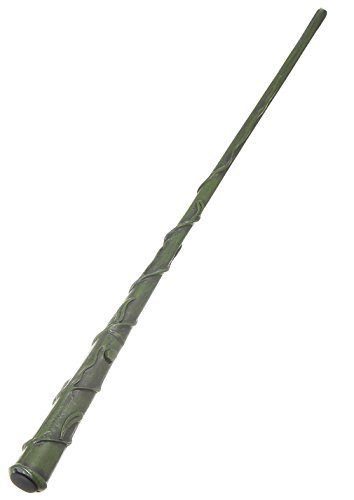
\includegraphics[scale=0.05]{magic.jpg}}
\renewcommand{\labelitemi}{\sign}

\begin{itemize}

\item Три простых рабочих мантии (черных)
\item Одна простая остроконечная шляпа (черная) на каждый день
\item Одна пара защитных перчаток
\item Один зимний плащ
\item Батильда Бэгшот, «Теория магии»
\item Адальберт Уоффлинг, «Пособие по трансфигурации для начинающих»
\item 1 волшебную палочку
\item 1 котел (оловянный стандартный размер №2)
\item 1 комплект стеклянных или хрустальных флаконов
\item 1 телескоп
\item 1 медные весы
\end{itemize}
\clearpage

\section{Список изучаемых предметов}
\begin{itemize}
\item Астрономия
\item Заклинания
\item Защита от тёмных искусств
\item Зельеварение
\item История магии
\item Травология
\item Трансфигурация
\item Полёты на мётлах
\end{itemize}
\end{document}